\chapter{Introduction}
\label{chp:chapter1}
\graphicspath{{figures/}{figures/chapter1/}}
\pgfplotsset{
    table/search path={{figures/chapter1/data},{data}},
}

Isogeometric analysis, introduced by Hughes et al.~\cite{HUGHES20054135}, leverages computer aided design (CAD) representations directly in finite element analysis. It has been shown that this approach can alleviate the model preparation burden of going from a CAD design to an analysis model and improve overall solution accuracy and robustness~\cite{bazilevs2006isogeometric, da2011some, da2014mathematical}. Additionally, the higher-order smoothness inherent in CAD basis functions make it possible to solve higher-order partial differential equations, e.g. the biharmonic equation~\cite{kapl_isogeometric_2015, kapl_isogeometric_2017}, the Kirchhoff-Love shell problem~\cite{kiendl2009isogeometric, kiendl2010bending, kiendl2015isogeometric} and the Cahn-Hilliard equation~\cite{gomez2008isogeometric, borden2014higher} directly without resorting to complex mixed discretization schemes.\par

CAD models are often built from collections of non-uniform rational B-splines (NURBS). Adjacent NURBS patches often have inconsistent knot layouts, different parameterizations, and may not even be physically connected. Additionally, trimming curves~\cite{kim2009isogeometric, schmidt2012isogeometric} are often employed to further simplify the design process and to extend the range of objects that can be modeled by NURBS at the expense of further complicating the underlying parameterization of the object. While usually not an issue from a design perspective, these inconsistencies in the NURBS patch layout, including trimming, must be accommodated in the isogeometric model to achieve accurate simulation results. As shown in Figure~\ref{fig:geometries}, two primary approaches are often employed. First, the exact trimmed CAD model, shown in Figure~\ref{fig:geometries} in the middle, is used directly in the simulation~\cite{schmidt2012isogeometric}. To accomplish this requires additional algorithms for handling cut cells and the weak imposition of boundary conditions and may result in reduced solution accuracy and robustness. Second, the CAD model is reparameterized~\cite{xu2014high}, as shown in Figure~\ref{fig:geometries} on the right, into a watertight spline representation like multi-patch NURBS, subdivision surfaces~\cite{peters2008subdivision}, or T-splines~\cite{sederberg_t-splines_2003} which can then be used as a basis for analysis directly. The reparameterization process often results in more accurate and robust simulation results but is only semi-automatic using prevailing approaches. In both cases, existing techniques are primarily surface-based due to the predominance of surface-based CAD descriptions.

\begin{figure}[ht]
	\captionsetup[subfigure]{labelformat=empty, font = footnotesize}
	\centering
	\begin{subfigure}[b]{0.32\textwidth}
		\centering
		\includestandalone[scale=.7]{geometry}
		\caption{A geometry}
	\end{subfigure}
	\begin{subfigure}[b]{0.32\textwidth}
		\centering
		\includestandalone[scale=.7]{trimmed_geometry}
		\caption{Trimmed model}
	\end{subfigure}
	\begin{subfigure}[b]{0.32\textwidth}
		\centering
		\includestandalone[scale=.7]{reparameterized_geometry}
		\caption{Reparameterized model}
	\end{subfigure}
	\caption{A geometry and two modelling strategies: trimming and reparameterization.}
	\label{fig:geometries}
\end{figure}

From the analysis perspective, the main challenge for conducting finite element analysis over a geometry consisting of multiple spline patches is how to efficiently and accurately exchange information among different patches. In this dissertation, we focus on the \textit{dual mortar method}, which can robustly apply constraints over intersections of reparameterized multi-patch geometries.  

\section{State of the art}

\subsection{Local refinable splines}

\begin{figure}[h]
    \centering
    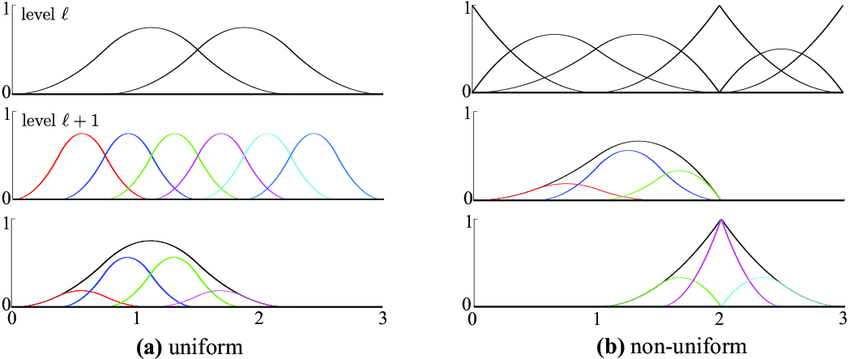
\includegraphics[width=.8\linewidth]{hierarchical-bsplines}
    \caption{Subdivision of B-spline basis functions: (a) Uniform, and (b) non-uniform B-spline basis functions are represented by linear combinations of refined basis functions~\cite{hennig2016bezier}.}\label{fig:hierarchical-bsplines}
\end{figure}

In 1988, Forsey and Bartels \cite{forsey_hierarchical_1988} introduced the hierarchical B-spline refinement algorithm, which can restrict the influence of refinement to the locality of interest. The algorithm is achieved by a re-representation process that replaces each basis function by an equivalent linear combination of a set of basis functions defined by nested knot vectors. However, due to the lack of a natural control grid, the hierarchical B-spline has not been widely recognized in the CAD society, and few applications can be found in geometric design. Recently, this technique has been extended to Isogeometric Analysis, by Vuong \textit{et al.} \cite{vuong_hierarchical_2011}. Owing to the construction strategy, the resulted hierarchical basis function are linearly independent and retain the maximal regularity, which renders the hierarchical B-spline a good candidate for analysis. The numerical tests demonstrate that the use of hierarchical B-splines lead to superior performance for problems with corner singularity. A subdivision-based hierarchical B-spline was proposed by Bornemann \textit{et al.} \cite{bornemann_subdivision-based_2013}, to tackle the intricate algorithms in the software implementation of hierarchical B-splines. The subdivision scheme (see Figure.~\ref{fig:hierarchical-bsplines}) establishes algebraic relations between the basis functions and their coefficients defined on different refinement level of the mesh and greatly ease the implementation of hierarchical B-splines. Consecutively, the truncated basis for hierarchical splines was introduced by Giannelli \textit{et al.} \cite{giannelli_thb-splines:_2012}. It is created by eliminating from the coarse hierarchical basis function the contribution corresponding to the subset of finer basis functions. Besides all the nice properties of hierarchical B-splines, the truncated basis for hierarchical splines obtain smaller support and form a partition of unity, which leads to sparser matrices and lower condition numbers. \par

However, all the above hierarchical B-splines are still under the tensor product formulism, which restricts hierarchical B-splines to a global rectangular parametric domain. In order to represent complex topologies, subdivision schemes are widespread in geometry processing and computer graphics. Among the most popular subdivision schems are the Catmull-Clark \cite{catmull_recursively_1978}, Doo-Sabin \cite{doo_behaviour_1978} and Loop's \cite{loop_smooth_1987} scheme. For Isogeometric Analysis, Wei \textit{et al.} \cite{wei_truncated_2015} introduced truncated hierarchical Catmull-Clark subdivion that can handle extraordinary nodes involved in complex topologies. Truncated hierarchical Catmull-Clark subdivion inherits the surface continuity of Catmull-Clark subdivision, namely $C^1$ continuity at extraordinary points and $C^2$ continuity elsewhere. Loop subdivision surfaces provide similar regularity properties as truncated hierarchical Catmull-Clark subdivion and have been applied to Isogeometric Analysis in \cite{kang_truncated_2016,pan_isogeometric_2015} to generate triangular meshes. One of the limitations in the implementation of subdivision meshes is that the basis function around the extraordinary point is composed of piecewise polynomial functions with an infinite number of segments, which leads to insufficient integration by Gauss quadrature. To deal with this issue, various quadrature rules and adaptive strategies have been examined in \cite{nguyen_comparative_2014} for the Poisson problem on the disk and in \cite{juttler_numerical_2016} for fourth order partial differential equations. \par
\begin{figure}[h]
    \centering
    \begin{subfigure}[b]{0.45\textwidth}
        \centering
        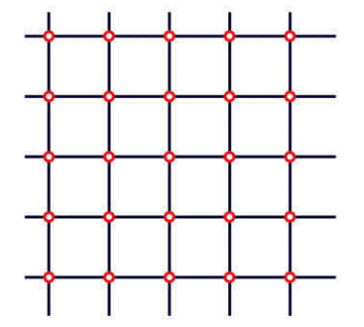
\includegraphics[width=\linewidth]{bspline-control-grid}
        \caption{B-splines}
    \end{subfigure}
    ~
    \begin{subfigure}[b]{0.45\textwidth}
        \centering
        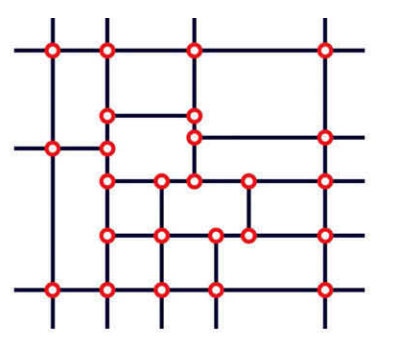
\includegraphics[width=\linewidth]{tspline-control-grid}
        \caption{T-splines}
    \end{subfigure}   
    \caption{Control points lie in a rectangular grid. (a) Topology of B-spline control grid. (b) Topology of T-spline
    control grid, the presence of T-junction control points is allowed~\cite{bazilevs_isogeometric_2010}.}\label{fig:Tspline-control-grid}
\end{figure}

\begin{figure}[h]
    \centering
    \begin{subfigure}[b]{0.45\textwidth}
        \centering
        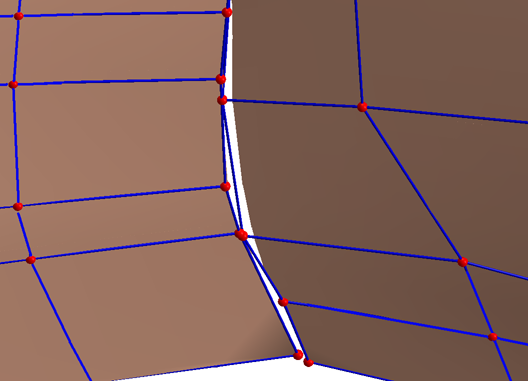
\includegraphics[width=\linewidth]{bspline-two-patch}
        \caption{B-splines}
    \end{subfigure}
    ~
    \begin{subfigure}[b]{0.45\textwidth}
        \centering
        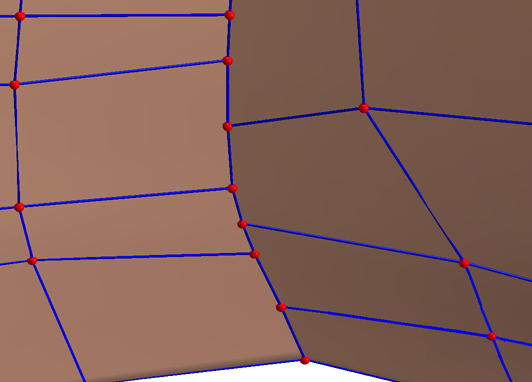
\includegraphics[width=\linewidth]{tspline-two-patch}
        \caption{T-splines}
    \end{subfigure}   
    \caption{A gap between two B-spline surfaces, fixed with a T-spline~\cite{sederberg_t-splines_2003}.}\label{fig:Tspline-two-patch}
\end{figure}

In 2003, Sederberg \textit{et al.} \cite{sederberg_t-splines_2003} introduced T-splines, which allow for the existence of T-junctions in the mesh, so that lines of control points need not traverse the entire mesh. Thus, local refinement can be realized by introducing T-junctions (see Figure.~\ref{fig:Tspline-control-grid}) around interested region. Since the concept of T-splines is a generalization of NURBS technology, it can also be used to merge NURBS surfaces that have different discretizaitons at the intersection (see Figure.~\ref{fig:Tspline-two-patch}). Due to the desirable features of T-splines, Bazilevs \textit{et al.} \cite{bazilevs_isogeometric_2010} explored this technology in Isogeometric Analysis, and numerical results demonstrated its potential for solving structural and fluid problems. By utilizing the B\'ezier extraction operator, a finite element data structure for T-splines \cite{scott_isogeometric_2011} were developed to ease the incorporation of T-splines into existing finite element codes. However, it has been proven \cite{buffa_linear_2010} that the original definition of T-splines is not sufficient to ensure the linear independence of the basis functions. To circumvent this issue, analysis suitable T-splines \cite{li_linear_2012} were developed by applying an additional constraint that no two orthogonal T-junction extensions are allowed to intersect. Subsequently, the mathematical properties of analysis suitable T-splines were studied in \cite{li_analysis-suitable_2013,xin_li_properties_2015}, and it has been sucessfully applied to the boundary element method \cite{scott2013isogeometric}. Meanwhile, an adaptive local h-refinement algorithm with T-splines and a local refinement of analysis-suitable T-splines were introduced by D\"{o}fel \textit{et al.} \cite{dorfel_adaptive_2010} and Scott \textit{et al.} \cite{scott_local_2012}, respectively. However, for both algorithm, the refined mesh is not as local as one would hope and this problem might be severe in 3D.\par

\subsection{Multi-patch geometrically continuous functions}

One of the advantages of Isogeometric Analysis is that it provides basis functions with high smoothness, \textit{i.e.} for $p$-th order splines, they enjoy up to $C^{p-1}$ continuity within a single patch. Thus, it is possible to directly discretize differential operators of order higher than 2. However, continuity higher than $C^0$ for multi-patch discretization imposes significant difficulties. The conception of geometric continuity is very important in CAD field \cite{peters_chapter_2002} for designing smooth multi-patch domain containing extraordinary points \cite{peters_joining_1992}. The parametric continuity requires both the smoothness of the geometry and its parameterization, while the geometric continuity only requires the smoothness of the geometry. Hence, the geometric continuity of order $s$ ($G^s$ continuity) is a weaker continuity constraint as compared to $C^s$ parametric continuity. It has been proved by Groisser and Peters \cite{groisser_matched_2015} that $G^s$ continuity in the parametric space is equivalent to $C^s$ continuity of the basis function after the parametric mapping. Thus, the construction of $C^s$ isogeometric basis functions in the physical space can be achieved by constructing $G^s$ in the parametric space. Bercovier \textit{et al.} \cite{bercovier_smooth_2014} has shown that for multi B\'ezier patches over an unstructured quadrilateral mesh, as long as the order of polynomial is high enough, there always exists the minimal determining set for a $C^1$ continuity construction. Moreover, the resulting basis functions do not contain subdivisions around extraordinary vetices.\par

The case of $G^1$ continuous functions on bilinearly parametrized two-patch B-spline domains was considered by Kapl \textit{et al.} \cite{kapl_isogeometric_2015}, where the $C^1$ basis functions are constructed and analyzed by numerical tests. It is shown that the space dimensionality heavily depends on the parameterization of two bilinear patch, and optimal convergence is observed on the biharmonic problem. However, over-constrained $C^1$ isogeometric spaces that cause sub-optimal convergence are also observed for certain configurations (\textit{e.g.} two-patch non-bilinear parameterizations and $C^{p-1}$ continuity within the patches for $p$-th order spline space). A theoretical analysis of the cause of this so-called $C^1$ locking phenomenon is provided in \cite{collin_analysis-suitable_2016}, where the analysis-suitable $G^1$ geometry parameterization, that allows for optimal approximation of $C^1$ isogeometric spaces, is identified and verified by numerical examples. The method in \cite{kapl_isogeometric_2015} has been extended to bilinearly parameterized multi-patch domains in \cite{kapl_isogeometric_2017}, where the simple explicit formulas for spline coefficients of $C^1$ basis function are derived and nested $C^1$ isogeometric spaces are generated. Recently, Kapl \textit{et al.} \cite{kapl_space_2017,kapl_space_nodate} explored the construction of $C^2$ isogeometric functions on multi-patch geometries and utilized the $C^2$ isogeometric spaces for $6$-th order PDE.\par
Although the geometrically continuous functions circumvent the use of subdivisions for domains with extraordinary vertices, the requirement of $C^0$ parameterization averts local mesh refinement, and lower continuity is required to avoid $C^1$ locking effect. Thus, its implementation can be complex and it may not be a potential candidate for analysis in more general situations.\par


\section{Research contributions}

\section{Organization of the dissertation}